\documentclass{article}
\usepackage[final]{neurips_2019}
\usepackage[utf8]{inputenc} % allow utf-8 input
\usepackage[T1]{fontenc}    % use 8-bit T1 fonts
\usepackage{url}            % simple URL typesetting
\usepackage{booktabs}       % professional-quality tables
\usepackage{amsfonts}       % blackboard math symbols
\usepackage{nicefrac}       % compact symbols for 1/2, etc.
\usepackage{microtype}      % microtypography
\usepackage{subfigure}
\usepackage{graphicx}

\setcitestyle{square,numbers,comma,sort&compress}

\usepackage[pagebackref=true,breaklinks=true,letterpaper=true,colorlinks,bookmarks=false,citecolor=blue]{hyperref}

\title{Design Choices for Invertible Neural Networks}


\author{%
  Max Daniels \\
  Northeastern University\\
  \texttt{daniels.g@northeastern.edu} \\
}

\begin{document}

\maketitle

\begin{abstract}
Invertible neural networks are an alternative to Generative Adversarial Networks which permit generative modeling through maximum likelihood estimation of the network parameters. Theoretically, these networks are fully invertible, but in practice their inverse map may be numerically challenging to compute. We take a deep dive investigation of the GLOW network to find one cause of this instability. We then test various remedies and demonstrate two options which solve the problem with no harm to network training. Finally, we identify and analyze a coincidental design feature of the INN and draw comparisons to other GAN architectures.
\end{abstract}


\section{Introduction}
Invertible Neural Networks (INNs) are a class of generative neural networks which have been proposed recently as alternatives to the Generative Adversarial Network (GAN) methodology. Both are useful for generative modeling of high dimensional data distributions for which many samples are available. It is typically difficult to estimate the density function of an arbitrary high dimensional distribution, and instead the GAN solves a simpler task: learning a low dimensional parametrization of an approximation of the data manifold. The method sacrifices access to a density function, in turn prohibiting parameter estimation through maximum likelihood. In exchange for this, it is simple and computationally efficient to generate approximate samples from the data distribution.

In contrast, INNs learn an invertible map between a representation space and a data space of equal dimension. These architectures are designed to have computationally tractable Jacobians so that a prior over the representation space may be pushed forward as a differentiable density function over the entire data space. In turn, INNs permit training by maximum likelihood. This method sacrifices expressiveness of the network in exchange for a tractable Jacobian and despite their clever design, INNs are still significantly more expensive than typical GANs to train and sample from.

We study INNs in the domain of image generation. One key difficulty is that the inverse map of a trained INN may be highly non-Lipschitz, so that for particular points in the representation space it is numerically impossible to compute. One solution is to clip intermediate activations so they remain small, but this introduces image artifacts like those in Figure \ref{fig:corruption}. In most generative neural networks, representation likelihood correlates to the quality of the corresponding output image, but surprisingly, we observe empirically that points near the origin are among the most difficult to sample. 
\begin{figure}
    \centering
    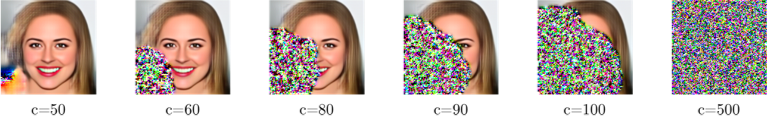
\includegraphics[width=\linewidth]{figures/figs.png}
    \caption{Corruption artifacts of a trained GLOW model when sampling the latent code $z=0$ using clipped intermediate activations. Under each image, the clipping parameter $c$ indicates the maximum allowed magnitude of any activation.}
    \label{fig:corruption}
\end{figure}

Recent work on the StyleGAN architecture highlights that large intermediate activations may be caused by unintended architectural flaws \cite{karras2019analyzing}. In light of this work, we assess the design of the GLOW architecture \cite{kingma2018glow}, a common instantiation of INNs, and pursue two main questions:
\begin{enumerate}
    \item Does the GLOW architecture have identifiable architectural oversights which cause large intermediate activations?
    \item How can the GLOW architecture be modified to reduce numerical challenges in computing the inverse map? 
\end{enumerate}

Through our experiments, we find the following:
\begin{enumerate}
    \item At a small scale, individual components of the GLOW architecture may cause large scale numerical problems while behaving as intended.  
    \item We suggest two methods to remedy this problem with minimal cost in terms of training effectiveness.
    \item We discover a hidden architectural characteristic which is necessary for stable inversion after training, motivating further investigation into the design of GLOW.
\end{enumerate}


\section{Experiments}

The GLOW architecture is organized in a series of flow steps, which are each individually invertible. In order to operate at multiple scales, the flow steps are connected by split and squeeze layers which manipulate the size and number of activation maps throughout the network. The flow steps are mainly responsible for image synthesis, by way of \textit{invertible 1x1 convolutions} as well as learned \textit{affine coupling layers}. We refer the reader to \cite{kingma2018glow} for more details.

\begin{figure}
    \centering
    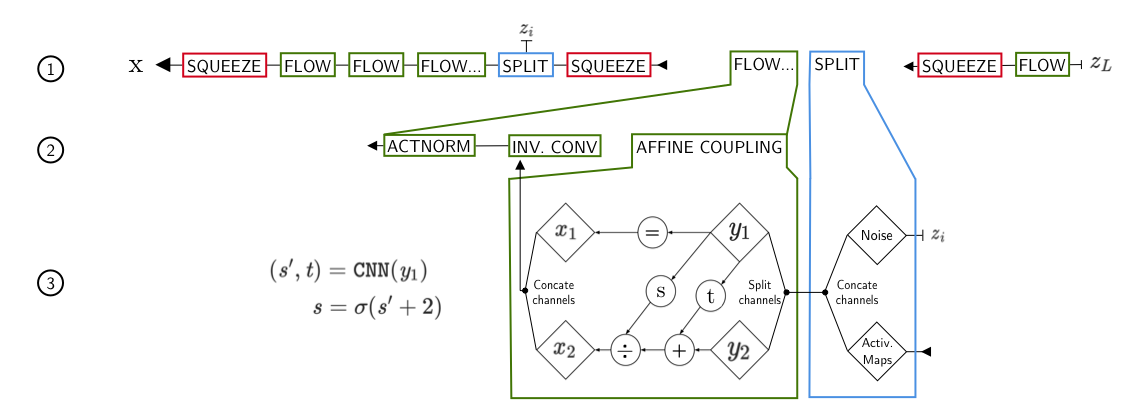
\includegraphics[width=\textwidth]{figures/Glow.png}
    \caption{A diagram of the GLOW architecture at multiple levels of granularity. Triangles indicate the points where intermediate activations enter and exit rows of the diagram. \textit{Row 1}: high level GLOW architecture. \textit{Row 2}: organization of an individual FLOW step. \textit{Row 3}: affine coupling uses a learned CNN to compute scale $s$ and bias $t$. Immediately following a SPLIT layer, $z_i$ is the input to CNN.}
    \label{fig:glow_architecture}
\end{figure}
In Figure \ref{fig:glow_architecture} we show the global organization of a GLOW network, along with an expansion of one flow step and, inside of it, an affine coupling layer. To identify the failure, we treat the GLOW model philosophically as a generator and inspect intermediate activations beginning with input noise and ending with an output image. 

Under this view, affine coupling plays a particularly important role. When noise is introduced into the INN in a split step, it is concatenated along the channel dimension as a contiguous block of noise activation maps. By coincidence, these noise channels are fed as input into the following affine coupling layer, which computes $s$ and $t$, the weights and biases for learned activation maps from the other channel block. The input noise is then forwarded to following layers with no transformation. From this analysis, we propose the following explanation for numerical instabilities:

\begin{quote}
Because affine coupling computes a divisor $s$, its output is required to be bounded away from zero. "Special" latent codes, such as those near the origin, are distribution shifted inputs which may induce outputs that violate this requirement.
\end{quote}

As an example, we study the first flow layer which receives noise input. As shown in Figure \ref{fig:sigma_plot}, as input noise concentrates around the origin, outliers of very low norm emerge.

\begin{figure}
    \centering
    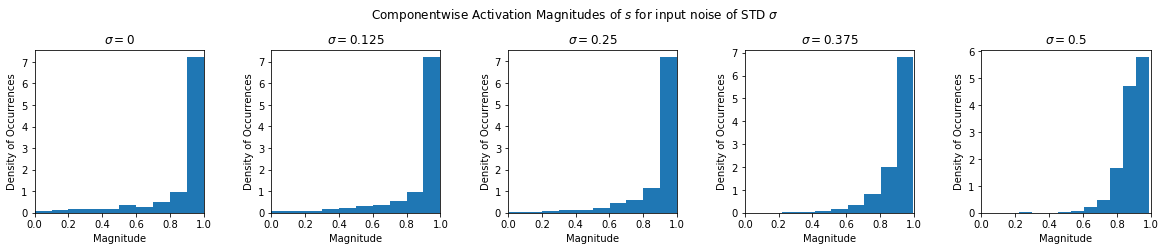
\includegraphics[width=\linewidth]{figures/s_plots.png}
    \caption{Empirical density functions of components of $s$ in the first FLOW layer which directly follows a SPLIT. As the input noise level is reduced, outliers emerge which cause large intermediate activations.}
    \label{fig:sigma_plot}
\end{figure}


\subsection{Architectural Remedies}
We consider four potential remedies to make affine coupling robust to distribution shifted input:
\begin{enumerate}
    \item Additive Coupling: this method, given in \cite{kingma2018glow}, simply fixes $s=1$. 
    \item Biased Sigmoid: add bias to the net output so it is bounded away from zero.
    \item Bounded Net: rather than biasing the output of the net, scale its output from $[0, 1]$ to $[a,b] \subseteq [0, 1]$.
    \item Randomized Splits: as part of the training procedure, GLOW internal activations are encouraged to follow a unit Gaussian distribution. Training an INN with random permutations of intermediate activation channels, inserted before each flow step, allows both noise input and intermediate activations to be used as input to affine coupling. This reduces the impact of distribution shifted input by mixing it with unit Gaussian activations.
\end{enumerate}

We show in Figure \ref{fig:train_performance} a comparison of training loss for these modifications. Replicating the results of \cite{kingma2018glow}, additive coupling noticeably harms training compared to affine coupling. The Biased Sigmoid and Bounded Net architectures exhibit training performance which is somewhat faster than GLOW with standard affine coupling. Randomized splits behave similarly to affine coupling.
\begin{figure}[h]
    \centering
    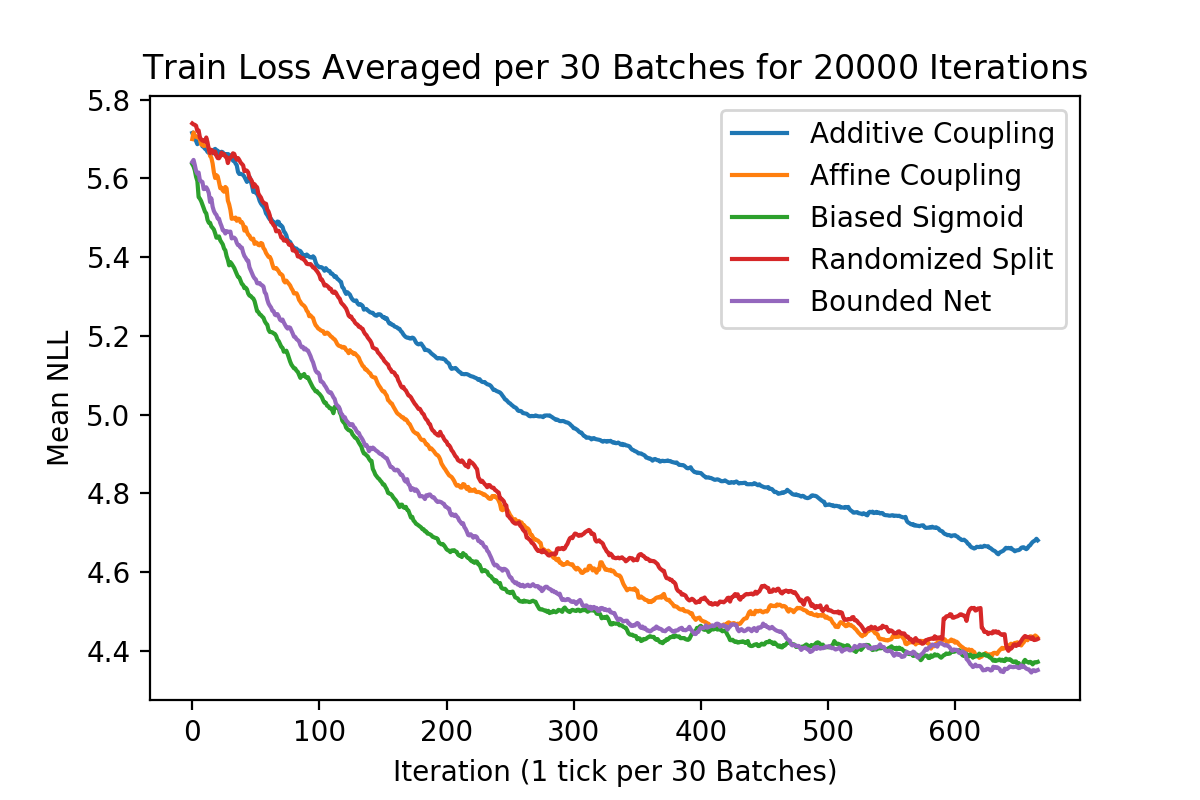
\includegraphics[width=0.6\linewidth]{figures/train_loss.png}
    \caption{Average training loss every $30$ batches while training a GLOW architecture with various architectural modifications. The unmodified control architecture uses affine coupling.}
    \label{fig:train_performance}
\end{figure}

After training, both the Biased Sigmoid and Bounded Net architectures have no sign of numerical instabilities. In contrast, the Randomized Splits architecture has significantly worse instability, as discussed in the following section.

\subsection{Randomized Splits and the "Noise Path"}

\begin{figure}
    \centering
    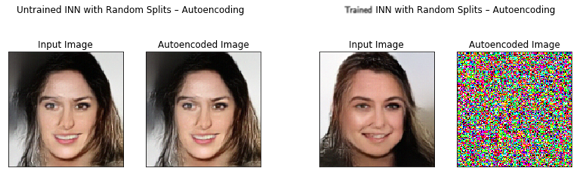
\includegraphics[width=0.8\linewidth]{figures/autoencode.png}
    \caption{After training, it is easy to map an image to a latent code, but impossible to invert the map. Here we show clipping at $c=50$, but behavior is the same for $c \in \{10, 20, 30, 40, 100, 500, 1000\}$.}
    \label{fig:autoencode}
\end{figure}
While it is easy to train a GLOW network with randomized splits, this architecture has significantly more instability. As shown in Figure \ref{fig:autoencode}, while the network architecture is capable of faithfully inverting images, as shown in the unlearned case, after learning it is impossible to sample even a partially uncorrupted image for a range of clipping parameters. Clearly, the allocation of noise to particular channels is crucial to the numerical stability of the inverse map, even if it bears little impact on training.


It is surprising that channel perturbations at the input to each flow layer should have negative effects, as channel permutation is a basic operation of the related RealNVP architecture \cite{dinh2016nvp}. This operation is generalized by GLOW through invertible 1x1 convolutions -- \textit{any channel permutation can be learned by the 1x1 convolution of any flow layer}. The key difference is whether this permutation is applied before or after affine coupling.

To speculate a cause for this, we highlight the similarity between affine coupling with concatenated noise input, and the AdaIN operation proposed for StyleGAN \cite{karras2018stylebased}. In both cases, noise is supplied to the network at multiple scales as input to a learned neural network which computes weights and biases of intermediate activations. In StyleGAN, these are the only source of stochastic input to the network, and they are responsible for controlling semantic characteristics of the output. 

Conceivably, the concatenation of input noise to fixed channels may induce a "noise path" which propagates the latent information of the representation throughout the network. Such a noise path would be disrupted by randomized splits. The accuracy of this interpretation, and the true role of noise concatenation in GLOW, are interesting directions for future work. 

\section{Conclusion}
The numerical stability of the GLOW architecture depends on the requirement that affine coupling layers compute scale coefficients $s$ for which each component is bounded away from zero. In the original GLOW architecture, this requirement is not enforced, so that affine coupling may cause large scale numerical problems while behaving as intended at a small scale. We examine multiple methods to enforce this requirement and find that the Biased Sigmoid and Bounded Net methods provide simple "plug-and-play" options which do not inhibit GLOW training.  This is a direct improvement over the Additive Coupling method considered in \cite{kingma2018glow}. Additionally, a third method using random channelwise permutations is shown to amplify the problem, a surprising result given that 1x1 invertible convolutions are explicitly designed to be able to learn arbitrary channelwise permutations. This gives evidence that the role of noise in image synthesis using the GLOW architecture is not fully understood, making it an interesting direction for future work.

\small

\nocite{karras2019analyzing}
\bibliography{citations} 
\bibliographystyle{plainnat}

\end{document}